\documentclass[a4paper,10pt]{article}

\usepackage[ngerman]{babel}
%\usepackage[top=3cm,bottom=3cm,left=3cm,right=3cm]{geometry} %NICHT IN KEMIE2


\usepackage{microtype} %schöneres typesetting  mit [stretch=10] für nur 1% anstelle von 2%
\usepackage{lmodern} %Latin Modern FONT
\usepackage{pifont} %schönere Font

\usepackage{chemfig}
\usepackage[version=4]{mhchem}
\usepackage{amsmath}
\usepackage{nicefrac}
\usepackage{amssymb}
%\usepackage{mathtools}

\usepackage{titlesec} %Um Section, etc bearbeiten zu können
\usepackage{fancyhdr}
\usepackage{setspace}
\usepackage{enumitem} %enumerate
\usepackage{arydshln} %für dashline
\usepackage{multicol}
\usepackage{lipsum}
\usepackage[labelfont=bf]{caption}

\usepackage[many]{tcolorbox}

%\usepackage{pgfornament} %Scheene Ornamente
\usepackage{witharrows} %Arrows in align-Umgebung
%\usepackage{awesomebox} %Notizboxen, etc
%\usepackage{textpos} %Für zum Beispiel vertikale Texte am Rand


%\usepackage{wrapfig} %Text um Bilder
%\usepackage{varwidth} % Alternative für engere minipage


\usepackage{hyperref}


\tcbuselibrary{theorems}

%\titlespacing*{\section}{0pt}{10mm}{3mm}
%\titlespacing*{\subsection}{0pt}{6mm}{3mm}
%\titlespacing*{\subsubsection}{0pt}{8mm}{3mm}


\renewcommand{\ttdefault}{lmtt} %Schriftart wird geändert zu Latin Modern Typewriter


\hypersetup{hidelinks,
			colorlinks=true,
			linkcolor=black,
			citecolor=miudiutex,
			urlcolor=miugray2
			}

\setlength\fboxsep{0pt}				
\setlength\columnsep{20pt}
\setlength{\parindent}{0pt}
\setcounter{section}{0}






%\definecolor{miudiutex}{HTML}{2f3d39}
\definecolor{miudiutex}{HTML}{1d2926}
\definecolor{miugray}{HTML}{b4cccf}
%\definecolor{miugray2}{HTML}{4d7365}
\definecolor{miugray2}{HTML}{6F8C81}
\definecolor{beige}{HTML}{F4F8D3}
\definecolor{white2}{HTML}{f5f7f8}
\definecolor{red}{HTML}{cf1f5c}
\definecolor{red2}{HTML}{9C191B}
\definecolor{green}{HTML}{00A36C}
\definecolor{delphinidin2}{HTML}{315794}
\definecolor{delphinidin}{HTML}{8B9EBA}
\definecolor{uniblau}{HTML}{004e9f}
\definecolor{unigelb}{HTML}{fcba00}
\definecolor{unigrau}{HTML}{909085}
\definecolor{pelargonidin}{HTML}{b33807}
\definecolor{pelargonidin2}{HTML}{FFDC96}
\definecolor{cyanidin}{HTML}{ba0746}
\definecolor{paeonidin}{HTML}{d15ca6}
\definecolor{petunidin}{HTML}{B88495}
\definecolor{petunitext}{HTML}{963354}
\definecolor{malvidin}{HTML}{8a2d8c}
\definecolor{mytheorembg}{HTML}{F2F2F9}
\definecolor{mytheoremfr}{HTML}{00007B}
\definecolor{uniblau2}{HTML}{27548A}
\definecolor{unigelb2}{HTML}{DDA853}
\definecolor{unidunkelblau2}{HTML}{183B4E}
\definecolor{unibeige}{HTML}{F5EEDC}


\tikzset{>=Latex}

\raggedcolumns %wichtig für Multicolumns
\color{miudiutex}



\usetikzlibrary{chains,
                positioning,
                shapes.multipart,
                }


\setchemfig
{%	
	bond offset=2pt,
	atom sep=15pt, 
	cram width=3pt,
	cram dash width=0.8pt,
	cram dash sep=1.2pt,
	double bond sep=2.5pt, 
	bond style={line width=1.1pt,cap=round},
	baseline=(current bounding box.center),
	bond join=true
}
\setcharge{extra sep=3pt}





%================================
% SYMBOLS
%================================

\newcommand{\RA}{$\rightarrow$~}
\newcommand{\RL}{$\rightleftharpoons$~}
\newcommand{\HARP}{\ding{226}~}
%$\xrightarrow{2}$ %Pfeil mit 2 drüber


%================================
% SHORT COMMANDS (BOXES ; ETC)
%================================


\newcommand{\info}[1]{\begin{note}{\color{miudiutex}#1}\end{note}}
\newcommand{\qsbig}[1]{\begin{qstion}{}{}\begin{center}
			#1 \end{center}\end{qstion}}
\newcommand{\notiz}[1]{\begin{notizz}{}{}\begin{center}
			{\color{miugray2!50!miudiutex}#1} \end{center}\end{notizz}}
\newcommand{\klausur}[1]{\begin{klausurinfo}{}{}\begin{center}
			#1 \end{center}\end{klausurinfo}}
\newcommand{\dfn}[1]{\begin{defin}{}{}\begin{center}
			#1 \end{center}\end{defin}}
\newcommand{\gesetz}[2]{\begin{gestex}{}{}\begin{center}
			#1 \end{center}\end{gestex}}
\newcommand{\gergesetz}[1]{\begin{gesgex}{}{}\begin{center}
			#1 \end{center}\end{gesgex}}
\newcommand{\klaausur}[1]{\begin{klausurinfo}[width=.77\linewidth]{}{}\begin{center}
			\footnotesize #1 \end{center}\end{klausurinfo}}
\newcommand{\winfo}[1]{\begin{wichtig}{}{} \begin{center}
#1 \end{center} \vspace*{0mm} \end{wichtig}}
\newcommand{\zit}[2]{\begin{zitat}{#1}{}\small #2 \end{zitat}}



\newcommand{\unten}{\end{center} \tcblower \begin{center}}


\newcommand*\circled[1]{\tikz[baseline=(char.base)]{
            \node[shape=circle,draw,inner sep=0.5pt,miudiutex] (char) {\tiny #1};}}
            
\newcommand{\miusquare}{{\color{miugray2!50}\scriptsize $\blacksquare$}~}
\newcommand{\miusquarp}{{\color{petunidin!50}\scriptsize $\blacktriangleright$}~}
\newcommand{\niu}{\item[\miusquare]}
\newcommand{\nip}{\item[\miusquarp]}
\newcommand{\mrk}[1]{{\color{petunitext!55!red}\textsc{#1}}}

%%%%% ABSAETZE

\newcommand{\pps}{\par \vspace*{1mm}}
\newcommand{\pp}{\par \vspace*{3mm}}
\newcommand{\ppbig}{\par \vspace*{8mm}}
\newcommand{\pphuge}{\par \vspace*{10mm}}



%================================
% HEADER & FOOTER FUER UNI
%================================
\newcommand{\miusfoot}{
\fancypagestyle{plain}{%
  \fancyhf{}%
  \renewcommand{\footrulewidth}{0.0mm}%
  \fancyfoot[L]{\hspace*{-3cm} {\color{miugray2}\textbf{\thepage}}}%
  \renewcommand{\headrulewidth}{0mm}%
} 
\pagestyle{plain}
}

\newcommand{\miushead}[2]{
\miusquare #1 - 4.Semester - ELW \hfill 
\includegraphics[width=60pt]{{F://LaTeX-Files/shiet/unibo}}
\par \vspace*{-3mm}
\hrulefill
\par \vspace*{1mm}
\par \vspace*{-4mm}
\normalsize	
	\begin{flushright}
	\textbf{\miusquare #2}\par \vspace*{1.5mm}
	\small	
	\textit{Letzte Überarbeitung:} \par 
	\footnotesize \today
	\end{flushright}
	\normalsize
\par \vspace*{-8mm}
}

\newcommand{\sidebar}{
\AddToHook{shipout/background}{
  \begin{tikzpicture}[remember picture,overlay, shift={(current page.south west)}]
   \path[fill=miugray2!15](0,0) rectangle (3.5cm,\paperheight);
%   \path[fill=miugray2!8](0,0) rectangle (3.5cm,\paperheight);
   \path[draw,miudiutex!50] (3.5,0) to (3.5,\paperheight);
%   \path[draw,miudiutex!50,dashed] (3.5,0) to (3.5,\paperheight);  
%   \node[opacity=0.8](a)at(12,10){\includegraphics[width=9cm]{F://LaTeX-Files/pngs/girl01}};
  \end{tikzpicture} 
}
}


\newcommand{\oddsidebar}{
\AddToHook{shipout/background}{
   \put(0in,-\paperheight){%
      \ifodd\value{page}\relax
           \begin{tikzpicture}[remember picture,overlay, shift={(current page.south west)}]
   \path[fill=miugray2!15](0,0) rectangle (3.5cm,\paperheight);
      \path[draw,miudiutex!50] (3.5,0) to (3.5,\paperheight);
  \end{tikzpicture}
      \else
           \begin{tikzpicture}[remember picture,overlay, shift={(current page.south east)}]
   \path[fill=miugray2!15](-3,0) rectangle (3cm,\paperheight);
%      \path[draw,miudiutex!50] (-3.5,0) to (-3.5,\paperheight);
  \end{tikzpicture}
      \fi
   }
}
}
%================================
% ENVIRONMENTS
%================================

\newenvironment{ctab}[2]{%
				\begin{spacing}{#1}
					\begin{center}
					\begin{tabular}{#2}}
					{\end{tabular}
					\end{center}
				\end{spacing}
				}


%================================
% Farbiger-Background-Box
%================================



\newcommand{\farbig}[1]{
\begin{tcolorbox}[%
				hbox,
				colback=miugray2!25,
				boxsep=-2pt,
				boxrule=0pt,
				arc=0pt,
				nobeforeafter,
				tcbox raise base,
				shrink tight,
				extrude by=1pt
				]
				{\color{miudiutex}{#1}}
\end{tcolorbox}~}

%================================
% SIMPLE SCHWARZER RAHMEN BOX
%================================


\newcommand{\boxfr}[1]{
	\begin{tcolorbox}[
	colframe=miugray2,
	colback=white!95!miugray2,
	boxrule = 0.5pt, 
%	toprule=0pt, bottomrule=0pt,rightrule=0pt,leftrule=0pt,
	boxsep=0pt,
	arc=4pt,
	drop shadow southeast,
	enhanced
	]
	\color{miudiutex}
	\begin{center}
	#1
	\end{center}
	\end{tcolorbox}
}

%================================
% Antwort-Box
%================================

\newcommand{\antwort}[1]{\par 
	\begin{tcolorbox}[
	colback=gray!15,
	breakable,
	enhanced,
	frame hidden,
	arc=5pt,
	boxrule = 2pt,
%	borderline west = {2pt}{0pt}{petunidin},
%	drop shadow=miugray2!30
	]
	\color{miudiutex}	#1
	\end{tcolorbox}
}

%================================
% Frame-IT
%================================

\newcommand{\frameit}[1]{\par 
	\begin{tcolorbox}[
	colback=gray!10,
	breakable,
	enhanced,
	frame hidden,
	arc=5pt,
	boxrule = 0pt,
	borderline west = {4pt}{0pt}{petunidin},
%	drop shadow=miugray2!30
	]
		#1
	\end{tcolorbox}
}



%================================
% Question BOX
%================================

\makeatletter
\newtcbtheorem{qstion}{Frage}{enhanced,
	breakable,
	colback=white,
	colframe=delphinidin!100,
%	capture=hbox,
	boxsep=-3pt,
	attach boxed title to top left={yshift*=-\tcboxedtitleheight},
	fonttitle=\bfseries,
%	title={#2},
	boxed title size=title,
	boxed title style={%
			sharp corners,
			rounded corners=northwest,
			colback=tcbcolframe,
			boxrule=0pt,
		},
	underlay boxed title={%
			\path[fill=tcbcolframe] (title.south west)--(title.south east)
			to[out=0, in=180] ([xshift=5mm]title.east)--
			(title.center-|frame.east)
			[rounded corners=\kvtcb@arc] |-
			(frame.north) -| cycle;
		},
	#1
}{def}
\makeatother



%================================
% SIMPLE Question BOX
%================================

\newcommand{\qssmall}{
\begin{tcolorbox}[hbox,colback=miugray2!55,boxsep=-4pt,boxrule=0pt,arc=2pt,nobeforeafter, tcbox raise base,shrink tight,extrude by=3pt]
\textbf{\color{white}{?}}
\end{tcolorbox}~~}

\newcommand{\folie}[1]{
\begin{tcolorbox}[%
				hbox,
				colback=miugray2!20,
				boxsep=2pt,
				boxrule=0.5pt,
				arc=2pt,
				nobeforeafter,
				tcbox raise base,
				shrink tight,
				extrude by=3pt]
				{\color{miudiutex}{Folie #1}}
\end{tcolorbox}~}


%================================
% NOTIZ BOX
%================================

\makeatletter
\newtcbtheorem{notizz}{Notiz}{enhanced,
	breakable,
	coltitle=white,
	colback=petunidin!10,
	colframe=petunidin!50,
	attach boxed title to top left={yshift*=-\tcboxedtitleheight},
	fonttitle=\bfseries,
%	title={#2},
	boxed title size=title,
	boxed title style={%
			sharp corners,
			rounded corners=northwest,
			colback=tcbcolframe,
			boxrule=0pt,
		},
	underlay boxed title={%
			\path[fill=tcbcolframe] (title.south west)--(title.south east)
			to[out=0, in=180] ([xshift=5mm]title.east)--
			(title.center-|frame.east)
			[rounded corners=\kvtcb@arc] |-
			(frame.north) -| cycle;
		},
		#1
}{def}
\makeatother



%================================
% Question BOX: Klausur
%================================

\makeatletter
\newtcbtheorem[no counter]{klausurinfo}{Klausurrelevant}{enhanced,
%	breakable,
	colback=miugray2!10,
	colframe=miugray2!75,
	attach boxed title to top left={yshift*=-\tcboxedtitleheight},
	fonttitle=\bfseries,
	title={#2},
	arc=4pt,
	boxrule=1pt,
	boxed title size=title,
	boxed title style={%
			sharp corners,
			rounded corners=northwest,
			colback=tcbcolframe,
			boxrule=0pt,
			arc=4pt,
		},
	underlay boxed title={%
			\path[fill=tcbcolframe] (title.south west)--(title.south east)
			to[out=0, in=180] ([xshift=5mm]title.east)--
			(title.center-|frame.east)
			[rounded corners=\kvtcb@arc] |-
			(frame.north) -| cycle;
		},
	#1
}{def}
\makeatother


%================================
% DEFINITION
%================================

\makeatletter
\newtcbtheorem[no counter]{defin}{Definition}{enhanced,
	breakable,
	colback=gray!10,
	colframe=gray,
	attach boxed title to top left={yshift*=-\tcboxedtitleheight},
	fonttitle=\bfseries,
	title={#2},
	arc=4pt,
	boxrule=1pt,
	fontlower=\footnotesize,
	collower=miugray2!50!miudiutex,
	boxed title size=title,
	boxed title style={%
			sharp corners,
			rounded corners=northwest,
			colback=tcbcolframe,
			boxrule=0pt,
			arc=4pt,
		},
	underlay boxed title={%
			\path[fill=tcbcolframe] (title.south west)--(title.south east)
			to[out=0, in=180] ([xshift=5mm]title.east)--
			(title.center-|frame.east)
			[rounded corners=\kvtcb@arc] |-
			(frame.north) -| cycle;
		},
	#1
}{def}
\makeatother

%================================
% Gesetzes-Text EU
%================================

\makeatletter
\newtcbtheorem[no counter]{gestex}{EU - Verordnung}{enhanced,
	breakable,
	colback=gray!10,
	colframe={gray!65!delphinidin},
	attach boxed title to top left={yshift*=-\tcboxedtitleheight},
	fonttitle=\bfseries,
	arc=4pt,
	boxsep=10pt,
	boxrule=1pt,
	fontlower=\footnotesize,
	collower=miugray2!50!miudiutex,
	boxed title size=title,
	overlay={%
			\node[xshift=-1cm,yshift=-1mm] at (frame.north east)
			{\includegraphics[width=8mm]{F://LaTeX-Files/shiet/eu}};
%			\node[draw,miugray2] at (frame.north) {{#2}}; 
			},%
	boxed title style={%
			sharp corners,
			rounded corners=northwest,
			colback=tcbcolframe,
			boxrule=0pt,
			arc=4pt,
		},
	underlay boxed title={%
			\path[fill=tcbcolframe] (title.south west)--(title.south east)
			to[out=0, in=180] ([xshift=5mm]title.east)--
			(title.center-|frame.east)
			[rounded corners=\kvtcb@arc] |-
			(frame.north) -| cycle;
		},
	#1
}{def}
\makeatother


%================================
% Gesetzes-Text Ger
%================================

\makeatletter
\newtcbtheorem[no counter]{gesgex}{Gesetzestext}{enhanced,
	breakable,
	colback=gray!10,
	colframe={gray!95!pelargonidin},
	attach boxed title to top left={yshift*=-\tcboxedtitleheight},
	fonttitle=\bfseries,
	title={#2},
	arc=4pt,
	boxrule=1pt,
	fontlower=\footnotesize,
	collower=miugray2!50!miudiutex,
	boxed title size=title,
	overlay={\node[xshift=-1cm,yshift=-3mm] at (frame.north east)
			{\includegraphics[width=8mm]{F://LaTeX-Files/shiet/ger}}; 
			},
	boxed title style={%
			sharp corners,
			rounded corners=northwest,
			colback=tcbcolframe,
			boxrule=0pt,
			arc=4pt,
		},
	underlay boxed title={%
			\path[fill=tcbcolframe] (title.south west)--(title.south east)
			to[out=0, in=180] ([xshift=5mm]title.east)--
			(title.center-|frame.east)
			[rounded corners=\kvtcb@arc] |-
			(frame.north) -| cycle;
		},
	#1
}{def}
\makeatother


%================================
% Question BOX: Wichtig
%================================

%\makeatletter
%\newtcbtheorem[no counter]{wichtig}{Wichtige Info}{enhanced,
%	breakable,
%	colback=pelargonidin2!80,
%	colframe=red2!100,
%	fonttitle=\bfseries,
%	title={#2},
%	leftrule=5mm,
%	boxed title size=title,
%	boxed title style={%
%			sharp corners,
%			rounded corners=northwest,
%			colback=tcbcolframe,
%			boxrule=0pt,
%		},
%	underlay boxed title={%
%			\path[fill=tcbcolframe] (title.south west)--(title.south east)
%			to[out=0, in=180] ([yshift=1mm,xshift=7mm]title.east)--
%			([yshift=1mm]title.center-|frame.east)
%			[rounded corners=\kvtcb@arc] |-
%			(frame.north) -| cycle;
%		},
%		watermark tikz={\draw[line width=2mm] circle (1.1cm)
%		node{\fontfamily{ptm}\fontseries{b}\fontsize{20mm}{20mm}\selectfont !};}],
%	attach boxed title to top left={xshift=5mm,yshift*=-\tcboxedtitleheight},
%	watermark zoom=0.65,
%	  underlay={%
%    \path[draw=none] (interior.south west) rectangle node[white]{\Huge \textbf{!}} ([xshift=-4mm]interior.north west);
%    },
%	#1
%}{def}
%\makeatother


\makeatletter
\newtcbtheorem[no counter]{wichtig}{Wichtige Info}{enhanced,
	breakable,
	colback=pelargonidin2!30,
	colframe=petunidin!100,
	fonttitle=\footnotesize\bfseries,
	title={#2},
	leftrule=4mm,
	boxed title size=title,
	boxed title style={%
			sharp corners,
			rounded corners=northeast,
			colback=tcbcolframe,
			boxrule=0pt,
		},
	underlay boxed title={%
			\path[fill=tcbcolframe] (title.south east)--(title.south west)
			to[out=180, in=0] ([yshift=2mm,xshift=-7mm]title.west)--
			([yshift=2mm]title.center-|frame.west)
			[rounded corners=\kvtcb@arc] |-
			(frame.north) -| cycle;
		},
		watermark tikz={\draw[line width=2mm] circle (1.1cm)
		node{\fontfamily{ptm}\fontseries{b}\fontsize{20mm}{20mm}\selectfont !};},
	attach boxed title to top right={yshift*=-\tcboxedtitleheight},
	watermark zoom=1.45,
	watermark opacity=0.35,
	  underlay={%
    \path[draw=none] (interior.south west) rectangle node[white]{\LARGE \textbf{!}} ([xshift=-4.3mm]interior.north west);
    },
    #1
}{def}
\makeatother





%================================
% ZITAT BOX
%================================

\tcbuselibrary{theorems,skins,hooks}
\newtcbtheorem{zitat}{Zitat}
{%
	enhanced,
	breakable,
	colback = gray!10!white,
	frame hidden,
	boxrule = 0sp,
	borderline west = {2pt}{0pt}{petunidin},
	sharp corners,
	detach title,
	before upper = \tcbtitle\par\smallskip,
	coltitle = gray!50!black,
	fonttitle = \bfseries\sffamily,
	description font = \mdseries,
	separator sign none,
	segmentation style={solid, gray!50!black},
}
{th}



\input{F://LaTeX-Files/shiet/vl.tex}
\usepackage{awesomebox}

\renewcommand{\arraystretch}{1.3}
%\setcounter{section}{1} % <--- FALLS KEINE SECTION DEFINIERT WIRD
\renewcommand{\textbf}[1]{\textsf{{\bfseries {#1}}}}

\begin{document}

\sidebar
\miushead{Vorlesung 20.05. \& 21.05. - PLMT}{Vorlesung 11 + 12}
\par \vspace*{5mm}
\section{Vorlesung 20.05.}
\subsection{Effekte von Temperatur}
\ppbig
\begin{center}
	\begin{tabular}{l|l}
\textbf{Temperaturerhöhung} & \textbf{Temperaturabsenkung} \\
\cline{1-2}
Abtöten von Mikroorganismen & Verringerung des Wachstums von Mikroorganismen \\ 
Beschleunigung chemischer Reaktionen & Verlangsamung chemischer Reaktionen \\
Denaturierung von Proteinen & Verringerung Enzymaktivität \\
Änderung des Aggregatzustandes & Änderung des Aggregatzustandes
\end{tabular}
	\end{center}	

\subsection{Einteilung von Mikroorganismen}
\ppbig

\begin{center}
\begin{tabular}{l|c|c|c}
 & \textbf{Minimum} &\textbf{Optimum} & \textbf{Maximum} \\
\cline{1-4}
psychrophil & -5 bis 5°C & 12-15°C & 15-20°C \\
psychrotolerant & 3-5°C & 20-30°C & 30-35°C \\
mesophil & 7-15°C & 30-40°C & 35-47°C \\
thermophil & 40-45°C & 55-75°C & 60-90°C \\
hyperthermophil &79-80°C & 80-90°C & 90-110°C \\
\end{tabular}
\end{center}



\subsection{Wiederholung Aktivierungsenergie}

\begin{figure}[h]
\centering
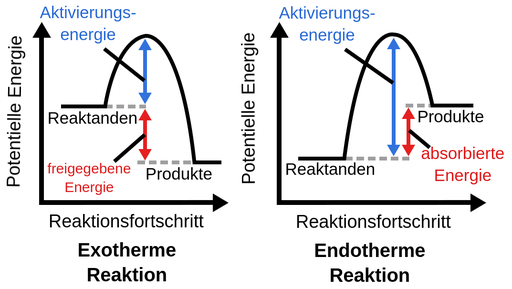
\includegraphics[scale=0.4]{endoexo}
\caption{Verschiedene Aktivierungsenergien}
\end{figure}

%\pagebreak

%\subsection{Begriffserklärungen für die Folien}

\textbf{Q10} ist der Faktor um den sich die Reaktionsgeschwindigkeit erhöht, wenn man die Temperatur um 10°C erhöht. \par
\textbf{Z-Wert} ist die Temperaturdifferenz, die benötigt wird um die Reaktionsgeschwindigkeit um den Faktor 10 zu erhöhen. \pp

\subsection{Effekte des Blanchierens}
\begin{itemize}
\item Inaktivierung der Enzyme
\item Elimination von Sauerstoff
\item Farbe
\item Reduktion der Keimbelastung
\item Schrumpfen bzw. Erweichen der Rohware
\item Entfernen von unerwünschten Aromastoffen
\end{itemize}
\pp

\subsection{Pasteurisation}

\klausur{pH 4,5 $>$ Pasteurisation \par pH 4,5 $<$ Sterilisation }

\pp
Im Folgenden wurden zwei Videos gezeigt über YouTube:\par 
\begin{center}
Tunnelpasteur-Video KHS INNOPAS \par 
JBT Hydromatic Hydrostatic Sterilizer
\end{center}

\subsection{Abtöten von Mikroorganismen}
\begin{figure}[h]
\centering
\begin{tikzpicture}
\draw[->] (0,0) to (0,4) node[right] {$N$};
\draw[->] (0,0) to (8,0) node[right] {$t$};
\draw[rounded corners=4pt] (0,3.5) .. controls (0.5,2) and (0.9,1) .. (2.5,0.5) .. controls (3.5,0.4) .. (5.5,0.3) to (8,0.2);
\end{tikzpicture}
\caption{Verlaufskurve Abtöten von Mikroorganismen}
\end{figure}

\ppbig

Kinetik erster Ordnung:
\begin{align*}
\frac{dN}{dt} = - k \cdot N
\end{align*}
Wobei $k$ die Reaktionsgeschwindigkeit in 1/s darstellt.
\par 
Für die Zahl der Mikroorganismen $N$ nach einer Zeit $t$ lässt sich folgende Formel aufstellen:
\begin{align*}
N(t) = N_0 \cdot e^{-k \cdot t}
\end{align*}

\pagebreak

\begin{figure}[h]

\begin{center}
\begin{tikzpicture}
\node[anchor=west] at (0,0){
\begin{tikzpicture}
\draw[->] (0,0) to (0,4) node[right] {$N$};
\draw[->] (0,0) to (4,0) node[right] {$t$};
\draw[-,miugray2] (0,3.5) to (3.5,0);
\draw (-0.1,3.5) node[left] {$10^6$} to (0,3.5);
\draw (-0.1,2.5) node[left] {$10^5$} to (0,2.5);
\draw (-0.1,1.5) node[left] {$10^4$} to (0,1.5);
\draw (-0.1,0.5) node[left] {$10^3$} to (0,0.5);

\draw (0,-0.1) node[below,scale=0.7] {1 min} to (0,0);
\draw (1,-0.1) node[below,scale=0.7] {2 min} to (1,0);
\draw (2,-0.1) node[below,scale=0.7] {3 min} to (2,0);
\draw (3,-0.1) node[below,scale=0.7] {4 min} to (3,0);
\draw [dashed,petunitext] (1,2.5) to (1,1.5);
\draw [<->, petunitext] (1,1.5) to node[below,scale=1,yshift=-2mm] {$D_t$}(2,1.5);
\end{tikzpicture} };
\node[anchor=west] at (6,0){
\begin{tikzpicture}
\draw[->] (0,0) to (0,4) node[right] {$D$ (min)};
\draw[->] (0,0) to (4,0) node[right] {$T$ (°C)};
\draw[-,miugray2] (0,3.5) to (3.5,0);
\draw (-0.1,3.5) node[left] {100} to (0,3.5);
\draw (-0.1,2.5) node[left] {10} to (0,2.5);
\draw (-0.1,1.5) node[left] {1} to (0,1.5);
\draw (-0.1,0.5) node[left] {0.1} to (0,0.5);

\draw (0,-0.1) node[below,scale=0.7] {60} to (0,0);
\draw (1,-0.1) node[below,scale=0.7] {70} to (1,0);
\draw (2,-0.1) node[below,scale=0.7] {80} to (2,0);
\draw (3,-0.1) node[below,scale=0.7] {90} to (3,0);
\draw [dashed,petunitext] (1,2.5) to (1,1.5);
\draw [<->, petunitext] (1,1.5) to node[below,scale=1,yshift=-2mm] {Z}(2,1.5);
\end{tikzpicture} };
\end{tikzpicture}
\caption{Linker Graph - Mikroorganismen über Zeit ; Rechter Graph D-Wert über Temperatur}
\end{center}

\end{figure}

\pp
Der \textbf{D-Wert} ist die Zeit, die man erhitzen muss, um die Keimzahl auf ein Zehntel zu reduzieren. \par 
Der \textbf{Z-Wert} ist die erforderliche Temperaturerhöhung, die nötig ist, um den D-Wert um eine Zehnerpotenz zu reduzieren
\ppbig
%\boxfr{
%\textbf{12D-Konzept:} \textit{Clostridium botulinum} muss 12 mal um ein Zehntel reduziert werden, damit es als abgestorben gilt. \textit{Clostridium botulinum} dient als Leitkeim für sichere Konserven nach dem 12D-Konzept
%}
\awesomebox[petunitext]{1mm}{\faExclamationTriangle}{miugray2}{\textbf{12D-Konzept:} \textit{Clostridium botulinum} muss 12 mal um ein Zehntel reduziert werden, damit es als abgestorben gilt. \textit{Clostridium botulinum} dient als Leitkeim für sichere Konserven nach dem 12D-Konzept}

\section{Vorlesung 21.05.}

\subsection{D-Wert}
Wie bereits in der letzten Vorlesung erwähnt, ist der \textbf{D-Wert} die Zeit, die man erhitzen muss, um die Keimzahl auf ein Zehntel zu reduzieren. Um den D-Wert für eine bestimmte Temperatur zu errechnen, können wir uns folgende Formel herleiten:

\begin{align*}
z &= \frac{T_2 - T_1}{\log(D_1) - \log(D_2)} \\
 &= \frac{T_2 - T_1}{\log(\frac{D_1}{D_2})} \\
\log(\frac{D_1}{D_2}) &= \frac{T_2 - T_1}{z} \\
\frac{D_1}{D_2} &= 10^{\frac{T_2 - T_1}{z}} \\
D_1 &= D_2 \cdot 10^{\frac{T_2 - T_1}{z}} 
\end{align*}

\pagebreak

\reversemarginpar
\subsection{F-Wert}
Der \textbf{F-Wert} ist definiert als die Summe aller letalen Effekte, die im Verlauf einer Erhitzung auf eine Mikroorganismen-Population wirken.
Der F-Wert beschreibt den Erhitzungseffekt, also die Keimabtötungsrate. Dabei geht man von folgendem Grundwert aus:
%\marginnote[Manchmal auch anders in Formelsammlungen: log$_1$ - log$_2$ = $\frac{log_1}{log_2}$]{}[3cm]
\pp
\begin{center}
1 F-Wert = 1 Minute bei 121°C
\end{center}

\pp
Zur Berechnung des jeweiligen F-Wertes nutzen wir folgende Formel:

\begin{align*}
F = D(\log N_0 - \log N(t) )
\end{align*}

\subsubsection{Beispielberechnung}
Vor der Sterilisation beträgt die Keimzahl 1 Spore \textit{Clostridium botulinum} pro Gramm Lebensmittel. Da \textit{Clostridium botulinum} ein gefährlicher Toxinbildner ist, wird das sogenannte 12-D-Konzept angewendet, um auf 10$^{-12}$ Sporen pro Gramm Lebensmittel zu reduzieren, um eine ausreichende Sicherheit zu gewährleisten.\par 
Im Ergebnis enthält dann jedes billionste Gramm des Lebensmittels noch eine überlebende Spore, oder bei 1000 g-Dosen noch jede milliardenste Dose. Aus diesen Werten für den Leitkeim \textit{Clostridium botulinum} (D-Wert: 0,2 min) und den Anforderungen ergibt sich:
\begin{align*}
F &= 0,2 ~\text{min} \cdot (\log (1) - \log (10^{-12})) = 2,4 ~\text{min}
\end{align*}
Daher müssen wir 2,4 min bei 121°C erhitzen um eine ausreichende Sicherheit des Lebensmittels zu gewährleisten.






\subsubsection{Letalitätswert}

\marginnote[Je kleiner der Letalitätswert, desto effektiver \pp L = 1 \RA 121°C bei 1min \par L = 0,1 \RA 121°C bei 0,1min]{}[0pt]
Der \textbf{Letalitätswert} $L$, auch Letalitätsrate oder Teil-F-Wert (F abgeleitet von Fahrenheit) genannt, gibt an, wie effektiv Mikroorganismen mit definierter Hitzeresistenz abgetötet werden, wenn sie eine Minute lang einer bestimmten Temperatur ausgesetzt werden.
\pp
In der Berechnung des konkreten Letalitätswertes bei der Untersuchung einer Probe spielen die Dezimale Reduktionszeit und der Z-Wert eine Rolle.
\pp
So lässt sich der L-Wert wie folgt berechnen:


\begin{align*}
L = \frac{F_0}{F_t} = \frac{D(121,1)}{D_t} = 10^{\frac{T-121,1}{z}}
\end{align*}


\subsubsection{Erhitzungsprozess}
\marginnote[L-Wert gilt für idealen Erhitzungsprozess]{}[0pt]
\begin{figure}[h]
\centering
\begin{tikzpicture}
\draw[->] (0,0) to (0,4) node[right] {$T$};
\draw[->] (0,0) to (8.5,0) node[right] {$t$};

\draw[petunitext] (0,0) .. controls (2.5,4) and (5.5,4)  .. (8,0) node[above,yshift=15mm,xshift=-6mm] {real};
\draw[miugray2] (2.5,0) to (2.5,3) node[below,xshift=15mm] {ideal} to (5.5,3) to (5.5,0); 
\end{tikzpicture}
\caption{Realer vs. Idealer Erhitzungsprozess}
\end{figure}

%\begin{zitat}{Wikipedia}{} \small Der Z-Wert ist ein Begriff, der bei der Berechnung der thermischen Absterbezeit von Mikroorganismen verwendet wird . Er gibt an, um wie viele Grad die Temperatur erhöht werden muss, um eine zehnfache (d. h. 1 log 10 ) Verringerung des D-Werts zu erreichen . Der D-Wert eines Organismus gibt die Zeit an, die in einem bestimmten Medium bei einer bestimmten Temperatur benötigt wird, um die Anzahl der Organismen um das Zehnfache zu reduzieren. Er ist nützlich, um die Wirksamkeit thermischer Inaktivierungen unter verschiedenen Bedingungen zu untersuchen, beispielsweise beim Kochen und Konservieren von Lebensmitteln. Der Z-Wert ist ein Maß für die Änderung des D-Werts bei variierenden Temperaturen und stellt eine vereinfachte Version der Arrhenius-Gleichung dar. Er entspricht z=2,303 RT T ref /E. [ 2 ]

%Der z-Wert eines Organismus in einem bestimmten Medium ist die Temperaturänderung , die erforderlich ist, damit sich der D-Wert um den Faktor zehn ändert, oder anders ausgedrückt: die Temperatur, die erforderlich ist, damit sich die thermische Zerstörungskurve um einen Logarithmuszyklus verschiebt . Er ist der Kehrwert der Steigung, die sich aus der Auftragung des Logarithmus des D-Werts gegen die Temperatur ergibt, bei der der D-Wert ermittelt wurde. Während der D-Wert die Zeit angibt, die bei einer bestimmten Temperatur benötigt wird, um 90 % der Organismen abzutöten, setzt der z-Wert die Resistenz eines Organismus gegenüber unterschiedlichen Temperaturen in Beziehung. Der z-Wert ermöglicht die Berechnung der Äquivalenz zweier thermischer Prozesse, sofern der D-Wert und der z-Wert bekannt sind.

%\end{zitat}






\end{document}
